%%==================================================================%%
%% Author : Abascal Fern�ndez, Patricia                             %%
%% Author : S�nchez Barreiro, Pablo                                 %%
%% Version: 1.2, 15/05/2013                                         %%
%%                                                                  %%
%% Memoria del Proyecto Fin de Carrera                              %%
%% Application Engineering/Generadores de C�digo C#                 %%
%%==================================================================%%

Esta secci�n detalla la secuenciaci�n de las plantillas de generaci�n ed c�digo creadas para implementar el algoritmo de la secci�on anterior. La Figura~\ref{app:fig:templates} muestra ficha secuenciaci�n.

\begin{figure}[!tb]
  \center
  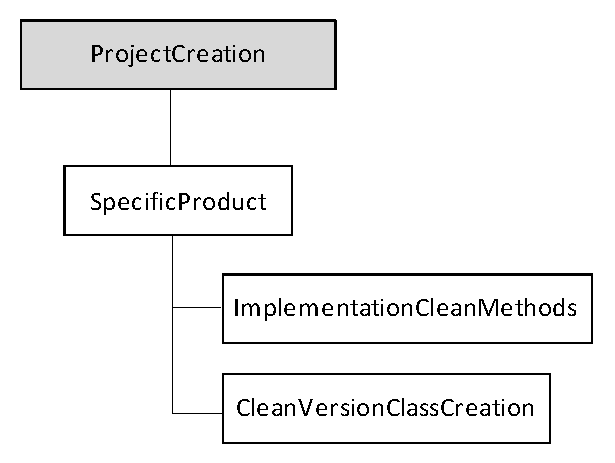
\includegraphics[width=\linewidth]{applicationEngineering/images/TemplatesAppEngineering.eps} \\
  \caption{Secuencia de ejecuci�n de las plantillas de generaci�n de c�digo (Ingenier�a de Aplicaciones)}
  \label{app:fig:templates}
\end{figure}

El punto de partida es id�ntico al utilizado para la fase de \emph{Ingenier�a del Dominio}; es decir, el generador de c�digo llamado \imp{ProjectCreation}, el cual crea el proyecto Visual Studio 2010 para el producto concreto. Este plantilla invoca a su vez a la plantilla \imp{SpecificProduct}, que es la que gobierna el proceso de generaci�n de c�digo a nivel de \emph{Ingenier�a de la Aplicaci�n}. Para ello, se invocan las siguientes plantillas:

%%=============================================================================================================================%%
%% NOTa(Pablo): Intenta aclarar esto, igual que hicimos para la fase de Inmgenier�a del Dominio                                %%
%%              y rearregla la figura                                                                                          %%
%%              Los que sean muy espec�ficos, te los cargas                                                                    %%
%%=============================================================================================================================%%

\begin{description}
   \item[\imp{MergeClasses}]. genera un listado de los paquetes del modelo y los paquetes directamente relacionados con los mismos.
   \item[ SpecificPath] genera un conjunto que incluye aquellos paquetes que necesitan ser implementado para el camino espec�fico seleccionado.
   \item[ExtractClassesAndOperations] genera un listado con cada paquete, por el camino espec�fico, y sus correspondientes clases y versiones clean de las operaciones que implementa.
   \item[FuseElements] fusiona las operaciones de las clases, con el mismo nombre, que est�n en paquetes diferentes.
   \item ImplementationCleanMethods] genera la implementaci�n final de los m�todos clean (con sus correspondientes implementaciones internas).
   \item[BranchFromSpecificProduct] extrae las versiones m�s profundas de cada m�todo en una rama concreta.
   \item[IsThereMethod] indica si un m�todo est� implementado en el paquete dado.
   \item[RearrangeMethods] selecciona de todas las ramas del proyecto espec�fico aquellas versiones de los m�todos m�s profundas y elimina las redundancias mediante el an�lisis de la alcanzabilidad.
   \item[SpecificMethods] genera la implementaci�n para la versi�n clean de cada clase y la implementaci�n interna de sus m�todos.
   \item[InternParams] genera los par�metros para las llamadas internas de los m�todos.
   \item[CleanVersionClassCreation] una vez creados los elementos a generar, esta plantilla genera la estructura completa del fichero resultante.
   \item[SpecificProductOperations] implementa funciones de uso recurrente a lo largo del resto de plantillas para simplificar el proceso. Entre las funciones implementadas est� la accesibilidad entre dos paquetes o la generaci�n de los paquetes para el caso espec�fico a analizar.
 \end{description}

Una vez implementados los generadores de c�digo para la fase de \emph{Ingenier�a de Aplicaci�n}, procedimos a realizar las pruebas pertinentes. 


